\section{The Idealized Prime+Probe Technique}

The Prime+Probe technique helps to visualize the vulnerability of AES Cipher during the 1st Round. To keep things simple, we'll consider an idealized environment in which only the attacking process and the victim encrypting process exists. Also assume that the attacking process will be able to invoke or interrupt the encrypting process at any time. Now since we are talking about triggered encryption, the plaintext is always known.

\begin{center}
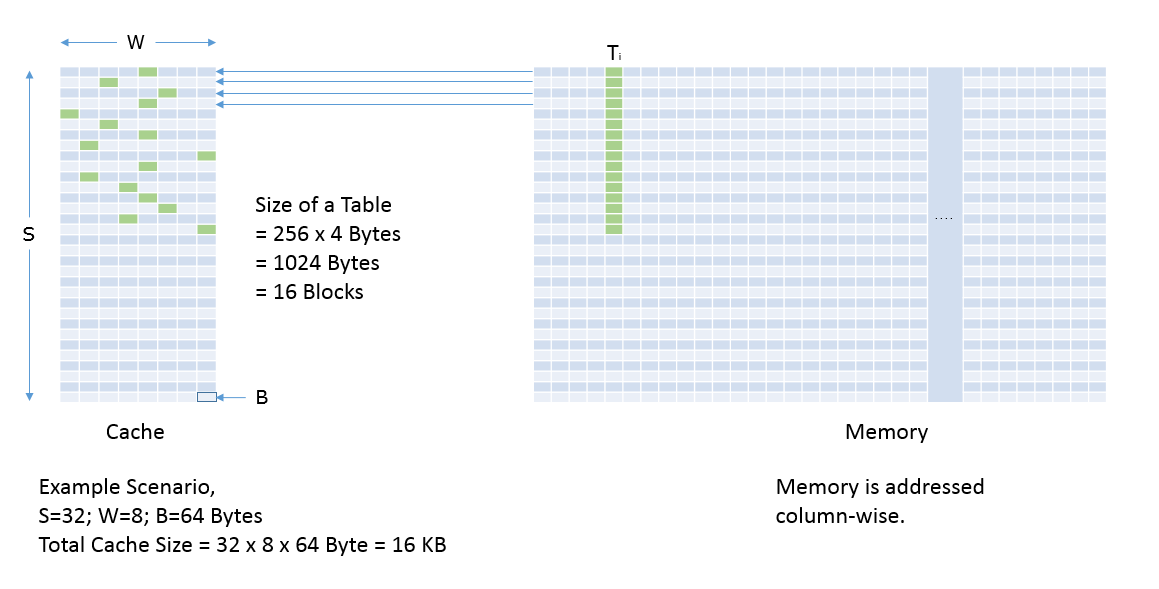
\includegraphics[scale=0.4,natwidth=1159,natheight=589]{Figures/lookup(new).png}
\captionof{figure}{Demonstration of how AES Lookup Table fits in memory and cache. On the left side, number of rows implies total number of cache sets, whereas, number of columns implies associativity of the cache. On the right side, instead of depicting memory as a continuous array of blocks, it is portrayed in congruence with cache memory. Note that all blocks in a row of memory competes for the blocks of corresponding row in cache memory. }
\label{fig: Demonstration of how AES Lookup Table fits in memory and cache.}
\end{center}

\begin{flushleft}
The Prime+Probe technique has the following 3 phases:
\end{flushleft}

\begin{itemize}
\item Prime
\item Trigger
\item Probe
\end{itemize}

\paragraph{Prime}
During the Prime phase, the Cache is filled completely by the attacking process. This can be done by allocating a contiguous amount of memory as big as the size of the cache and performing a read on it. If $S=32$, $W=8$ and $B=64$ Bytes, then

\begin{center}
Total size of the cache $=S\cdot W \cdot B=16$ KB
\end{center}

As implied by the figure above, performing a serial read on a contiguous memory as big as the cache results in inception of filling the cache. Continuing this way, we'll end up filling the cache completely after the reading is finished.

\paragraph{Trigger}
With the Cache filled with our data, we're in a position to invoke the encrypting process and trigger an encryption of some known plain text. As the encrypting process reaches the First Round and performs the first lookup, it is interrupted. An important point to note here is, we're idealizing the model to illustrate the susceptibility of the First Round. Recovering the AES Encryption Key is not the actual intent of this paper.

\begin{center}
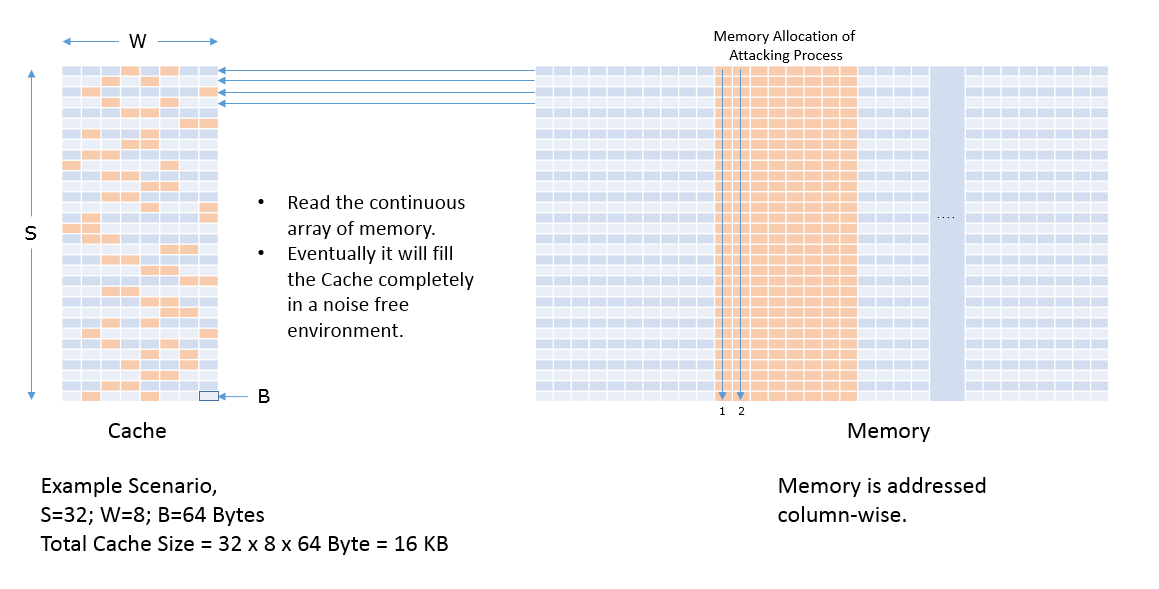
\includegraphics[scale=0.4,natwidth=1159,natheight=589]{Figures/filling(new).png}
\captionof{figure}{Demonstration of the Cache filling process. Note that reading continuous array of memory will cause allocation of one block from each cache set and due to Principle of Locality, immediate next read cycle will cause allocation of another block (different from the previous) from each cache set.}
\label{fig: Demonstration of the Cache filling process.}
\end{center}


\paragraph{Probe}
After we interrupt the encrypting process just after it performed its first lookup during the First Round of AES, we perform the Prime again, i.e. we fill the cache again. But this time, we maintain a clock measuring of how long it takes to read a \emph{memory block}. Before the Trigger phase, the cache was completely filled by our data. But after that Trigger phase, one block of the 
Lookup table $T_0$ is now in the cache due to the lookup operation. So all but that block will suffer from a cache miss.

\begin{center}
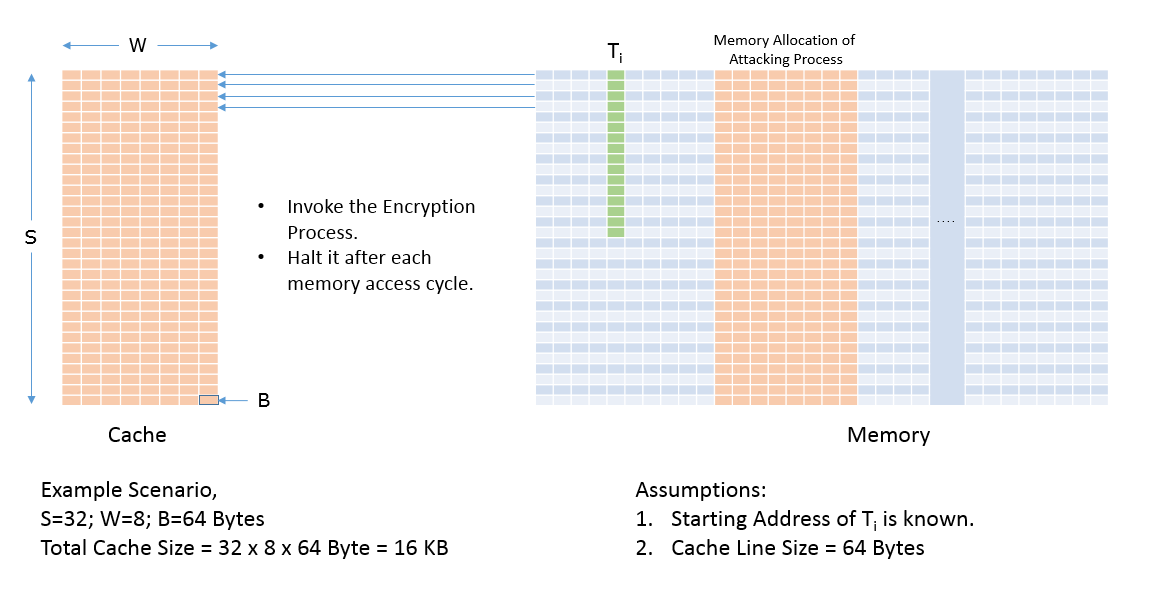
\includegraphics[scale=0.4,natwidth=1159,natheight=589]{Figures/prime(new).png}
\captionof{figure}{Demonstration of the Prime phase where reading a continuous array of memory equal to the size of the cache will eventually fill the cache completely with attacker's data in a noiseless environment.}
\label{fig: Demonstration of the Prime phase.}
\end{center}

Observing the position of the cache miss, we can easily identify which block of $T_0$ was accessed since we assumed Lookup Tables $T_i$ to be congruent with the cache. Now if we can identify which block of $T_0$ was accessed during the First Round, we can extract some valuable piece of information. Since size of \emph{memory block} is 64 Bytes, each \emph{memory block} holds 16 entry of the Lookup Table. So for example, if 7th block of $T_0$ was accessed, we can conclude the index $x_0^{(1)}$ was somewhat between 0x60 and 0x6F, i.e. high nibble is 0x6. We know

\begin{align*}
x_0^{(1)}=x_0^{(0)} \oplus k_0^{(0)}
\end{align*}

\begin{center}
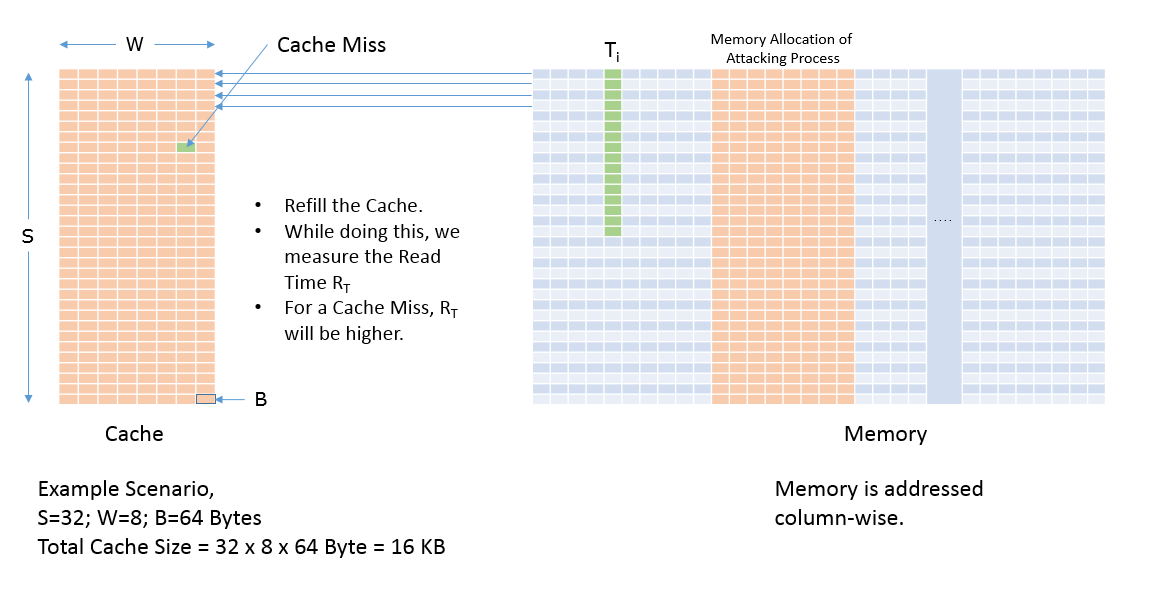
\includegraphics[scale=0.4,natwidth=1159,natheight=589]{Figures/probe(new).png}
\captionof{figure}{Demonstration of how information about the location of the cache miss during first round reveals critical information about the encryption key. In the example scenario, the high nibble of a Byte (0x6) is easily gleaned.}
\label{fig: Demonstration of the Probe phase.}
\end{center}

Here $x_0^{(0)}$ is the 1st Byte of the plaintext and $k_0^{(0)}$ is the 1st Byte of the Encryption Key. Now, since addition and subtraction in Galois Field are the same XOR operation, rearranging the equation yields:
\begin{align*}
k_0^{(0)}=x_0^{(0)} \oplus x_0^{(1)}
\end{align*}

Because we know $x_0^{(0)}$ from the plain text and the high nibble of $x_0^{(1)}$ from the Prime+Probe technique, we can compute the high nibble of the first Byte of the Encryption Key by a simple XOR operation. Proceeding this way for every Bytes $x_i^{(1)}$ for $i=0,1,2,...,15$, we can calculate $k_i^{(0)}$ for $i=0,1,2,...,15$ and dig up half of the Encryption Key. The idealized procedure is summarized in algorithm 1.

\begin{algorithm}
\caption{Abstract procedure for capturing half of the Key during the First Round}
\label{Abstract procedure for capturing half of the Key during the First Round}
\begin{algorithmic}[1]
	\State triggerEncryption()
	\For{$i \gets 0$ to $15$}
		\State fillCache()
		\State haltEncryption()
		\State $j \gets$ missedBlockIndex()
		\State $j \gets j\ll 4$
		\State $k_i^{(0)} \gets j \oplus x_i^{(0)}$\Comment{$k_i^{(0)}$ and $x_i^{(0)}$ resemble i-th Byte of the key and known plaintext respectively}
	\EndFor
\end{algorithmic}
\end{algorithm}
